\chapter{Metodologia de Desenvolvimento}
\label{chap:metodologia}

Neste capítulo detalha-se o trabalho proposto por essa monografia, um estudo sobre a utilização das instâncias EC2 F1 como recurso didático para a disciplina de Sistemas Eletrônicos Digitais Reconfiguráveis (SEDR) do curso de Engenharia de Computação da Universidade Federal do Ceará. Serão apresentadas a metodologia utilizada, todas as práticas realizadas e as ferramentas utilizadas.

\section{Metodologia Utilizada}\label{sec: metodologia-utilizada}

A metodologia adotada para a execução deste trabalho é mostrada nas etapas mostradas da Figura \ref{fig:metodologia}:



\begin{figure}[htb!] 
   	    \captionsetup{width=15cm}%Da mesma largura que a figura
		\Caption{\label{fig:metodologia}{Metodologia}}
		\UFCfig{}{
			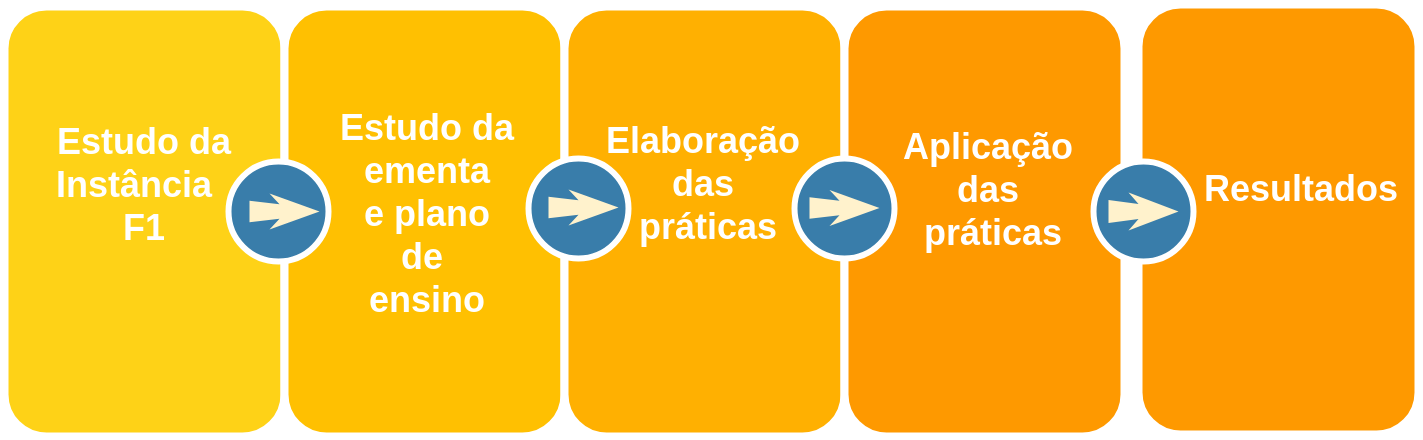
\includegraphics[width=16cm]{figuras/metodologia.png}
		}{
			\Fonte{Próprio Autor.}
	}		
\end{figure}
    
\begin{enumerate}
    \item \textbf{Estudo da Instância F1:} Primeiramente, foi realizado um estudo das instâncias EC2 F1 com o intuito de identificar as possibilidades que esse recurso poderia oferecer para o seu uso no ensino de FPGA.
    
    \item \textbf{Estudo da ementa e plano de ensino da Disciplina de SEDR:} Em seguida, deu-se início ao estudo da ementa e do plano de ensino da disciplina de SEDR para que a utilização das instâncias EC2 F1 fosse adequada da melhor forma possível ao plano de ensino.
    
    \item \textbf{Elaboração das práticas:} Baseando-se nos estudos já realizados e na documentação da Amazon Web Services, as práticas de laboratório foram idealizadas de forma a oferecer um conhecimento geral do processo de desenvolvimento de aplicações para FPGA com o serviço EC2 F1.
    
     \item \textbf{Criação da máquina virtual:} Com a finalidade de abordar o desenvolvimento local (\textit{on-premises}) com o kit de desenvolvimento da AWS \cite{on-premises} nas práticas 3 e 4, uma máquina virtual foi criada e configurada para conter o kit de desenvolvimento da AWS, o HDK e o SDK, e o ambiente de desenvolvimento da Xilinx SDSoC 2017.1 op, que contém o Vivado com uma licença específica para a FPGA Virtex UltraScale+ VU9P.
    
    \item \textbf{Aplicação das práticas:} Após a elaboração e testes das práticas, iniciou-se a fase de aplicação em laboratório.
    
    \item \textbf{Resultados:} Finalmente, nesta última etapa da metodologia foi analisada a eficácia do uso das instâncias EC2 F1, como recurso didático para a disciplina de SEDR, através da aplicação das práticas, e de análise de questionários respondidos pelos alunos ao final de cada prática.
	  
\end{enumerate}

  
\section{Contextualização}\label{sec: contextualizacao}

O trabalho foi realizado no Departamento de Teleinformática da Universidade Federal do Ceará. As práticas foram aplicadas em dois laboratórios deste mesmo departamento para alunos de graduação.

As práticas foram aplicadas na disciplina de SEDR, que é um componente optativo da estrutura curricular do Curso de Graduação em Engenharia de Computação e é ofertada no sétimo semestre da graduação, tendo a carga horária de 64 horas (vide ANEXO \ref{an:ex_anexo_a}) e tinha o total de 11 alunos matriculados. Dos quais, 2 alunos realizaram o trancamento da disciplina, 1 é a autora deste trabalho e, portanto, 8 alunos realmente realizaram as práticas. 

De acordo com a ementa, a carga horária total da disciplina é dividida igualmente entre teoria e prática, ou seja, são utilizadas 32 horas para a teoria e 32 horas para a pŕatica. A carga horária reservada para a  aplicação das práticas desenvolvidas neste trabalho foi de 10 horas, dessa quantidade, 2 horas foram utilizadas para uma aula teórica sobre a Amazon Web Services (AWS) e o serviço EC2 F1 e as 8 horas restantes foram reservadas para a aplicação das práticas, levando em consideração apenas as atividades desenvolvidas no laboratório durante o horário da aula.

As práticas foram realizadas no Laboratório de Informática e no Laboratório de Hardware do Departamento de Teleinformática. No primeiro, foram realizadas as práticas 1 e 2 que usam o acesso remoto às instâncias F1. As práticas 3 e 4 foram realizadas no Laboratório de Hardware, onde foram instaladas imagem das máquinas virtuais que permitem  o desenvolvimento local (\textit{on premises}) das práticas.

\section{Ferramentas Utilizadas}\label{sec: ferramentas}

Esta Seção detalha as ferramentas que foram utilizadas para a realização das atividades de labotório.

\subsection{Software}\label{sec: software}

\subsubsection{AWS Command Line Interface (CLI)}\label{sec: aws-cli}

A AWS \textit{Command Line Interface} (CLI) é uma ferramenta de código aberto que fornece comandos para interagir com os serviços da Amazon Web Services \cite{awscli}. Após a sua configuração, é possível gerenciar todos os recursos fornecidos pela AWS, pois é fornecido o acesso direto a APIs públicas de serviços da AWS. Esse acesso pode ser realizado por meio de comandos ou scripts de shell, ou até mesmo com programas em várias linguagens de programação, utilizando o SDK da AWS. Neste projeto, utilizou-se a AWS CLI para a iniciar instâncias pelo terminal, criar \textit{buckets} no S3 e armazenar o DCP gerado nesses \textit{buckets}.   

\subsubsection{GitHub}\label{sec: github}
o GitHub é uma plataforma de hospedagem de código-fonte que  utiliza o sistema de controle de versão distribuído Git. Ele é usado para armazenar o código-fonte de um projeto e rastrear o histórico completo de todas as alterações feitas nesse código. Além disso, é amplamente utilizado para divulgação e/ou contribuição de trabalhos. O GitHub foi utilizado neste trabalho para armazenar as alterações feitas pelos alunos no repositório da AWS, para que posteriormente o projeto modificado pudesse ser copiado para a máquina em que a prática estava sendo desenvolvida.

\subsubsection{Vivado Design Suite}\label{sec: vivado}
O Vivado Design Suite é um pacote de software produzido pela Xilinx que permite a edição, síntese, análise e simulação de um projeto para FPGA. Ele foi usado neste trabalho para o desenvolvimento dos projetos de FPGAs abordados nas práticas.

\subsubsection{VMware}\label{sec: vmware}

VMware um software/máquina virtual que permite a instalação e utilização de um sistema operacional dentro de outro \cite{vmware}. A fim de abordar o desenvolvimento \textit{on premises} usando os recursos da AWS, criou-se uma máquina virtual que continha todas as ferramentas, com suas devidas licenças, todas gratuitas,instaladas. O VMware foi utilizado para executar essa máquina virtual criada.

\subsection{Hardware}\label{sec: Hardware}

Utilizou-se os computadores do Laboratório de Informática, com sistemas operacional Linux, e o os computadores do Laboratório de Hardware com o sistema operacional Windows instalado.


\section{Estrutura das aulas de laboratório}
Como apresentado na Seção \ref{sec: contextualizacao}, as práticas 1 e 2 foram realizadas no Laboratório de Informática, utilizando as máquinas do próprio laboratório para fazer o acesso remoto às instâncias da AWS. Durante essas práticas os alunos acessam, via SSH da máquina local, a instância t2.2xlarge para desenvolverem seu projeto, gerar o DCP e criar a AFI, a ser gravada na FPGA. Após isso, a instância f1.2xlarge, a qual contém a placa com a FPGA, é acessada via ssh e finalmente, a AFI é gravada na FPGA conectada à instância. A Figura \ref{fig:praticas-1e2} mostra o procedimento descrito.

Para a realização das práticas 3 e 4 utilizou-se uma máquina virtual para realizar o desenvolvimento local. Nessa máquina, foram executados os comandos necessários para a criação e simulação do projeto, no caso da prática 3. Na prática 4 os comandos executados realizaram a simulação, a síntese e a conexão com a interface Shell. As Figuras \ref{fig:pratica3} e \ref{fig:pratica4} mostram a estrutura das práticas 3 e 4, respectivamente.

\begin{comment}
\begin{figure}[htb!] 
   	    \captionsetup{width=6cm}%Da mesma largura que a figura
		\Caption{\label{fig:praticas-1e2} Estrutura das práticas 1 e 2.}
		\UFCfig{}{
			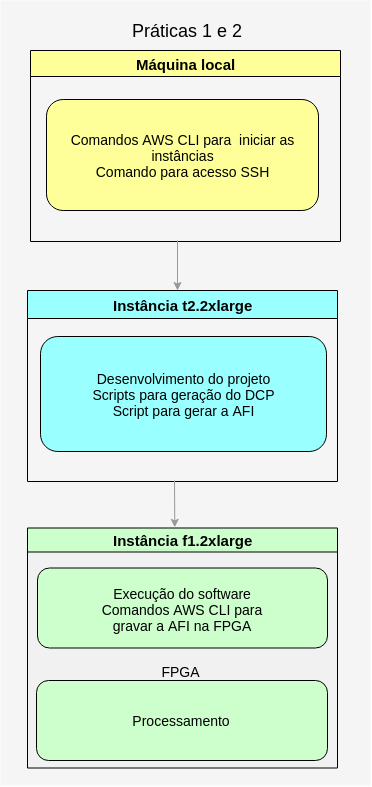
\includegraphics[width=7cm]{figuras/Praticas1e2.png}
		}{
			\Fonte{Próprio Autor.}
	}		
\end{figure}

\begin{figure}[htb!] 
   	    \captionsetup{width=7cm}%Da mesma largura que a figura
		\Caption{\label{fig:pratica3} Estrutura da prática 3.}
		\UFCfig{}{
			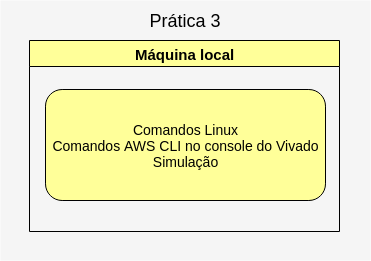
\includegraphics[width=8cm]{figuras/pratica3.png}
		}{
			\Fonte{Próprio Autor.}
	}		
\end{figure}

\begin{figure}[htb!] 
   	    \captionsetup{width=7cm}%Da mesma largura que a figura
		\Caption{\label{fig:pratica4} Estrutura da prática 4.}
		\UFCfig{}{
			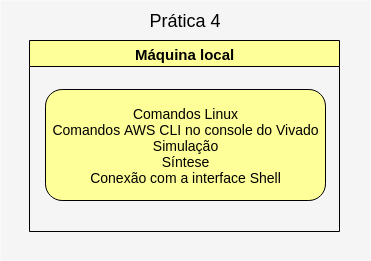
\includegraphics[width=8cm]{figuras/pratica4.png}
		}{
			\Fonte{Próprio Autor.}
	}		
\end{figure}
\end{comment}

\begin{figure}[h!]
\begin{minipage}{0.48\columnwidth}
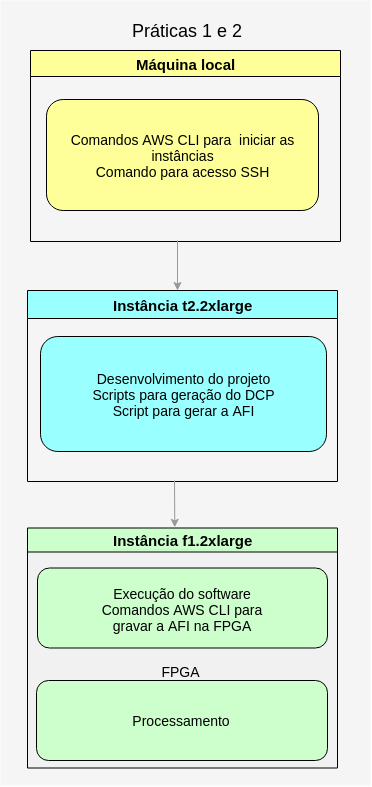
\includegraphics[width=\columnwidth,height=150mm]{figuras/Praticas1e2.png}
\end{minipage}
\begin{minipage}{0.48\columnwidth}
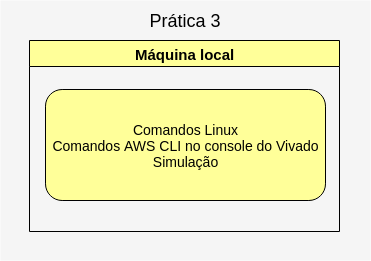
\includegraphics[width=\columnwidth,height=6cm]{figuras/pratica3.png}
\\[5mm]
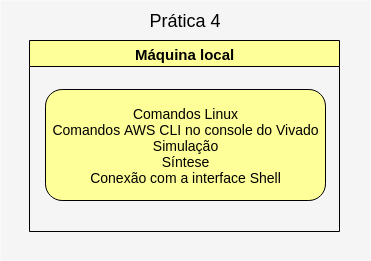
\includegraphics[width=\columnwidth,height=6cm]{figuras/pratica4.png}
\end{minipage}
\Fonte{Próprio Autor.}
\end{figure}



\section{Proposta de Práticas de Laboratório Para a Discplina de SEDR}

Após a realização de uma etapa de estudos sobre a utilização do serviço EC2 F1 da AWS, deu-se início ao estudo da ementa (vide ANEXO \ref{an:ex_anexo_a}) e do plano de ensino  da disciplina de SEDR, como citado na Seção \ref{sec: metodologia-utilizada}. Com base nesses estudos, foram propostas algumas práticas de laboratório que fossem factíveis, considerando-se limitações de tempo e de recursos financeiros para o acesso às instâncias da AWS, e que pudessem abordar o procedimento para o desenvolvimento de projetos em FPGA, na nuvem, de maneira satisfatória. Como resultado, chegou-se a um conjunto de quatro práticas que serão descritas a seguir. Maiores detalhes das práticas podem ser vistos nos roteiros de cada uma, disponíveis no Anexo deste documento e na plataforma GitHub, no link: \url{https://github.com/vanros/Praticas-SEDR-AWS}.

\subsection{Prática 1: Criação de uma Amazon FPGA Image (AFI) do exemplo CL hello world}

\noindent\textbf{\textit{Objetivo}}

O objetivo dessa prática foi apresentar o uso do serviço EC2 F1 da AWS, abordando a conexão e configuração das instâncias t2.2xlarge e f1.2xlarge, além de todos os procedimentos necessários para a execução de um projeto exemplo utilizando a FPGA conectada à instância f1.2xlarge.


\noindent\textbf{\textit{Breve descrição}}

Nesta prática foi utilizado um exemplo do repositório da AWS para realizar o procedimento de geração do DCP,  geração da AFI e a execução do software que se comunica com a FPGA. Nesse exemplo, o valor 0xEFBEADDE é escrito em um registrador, após isso a FPGA ler o mesmo registrador, realiza um \textit{byte swap}, alterando o valor para 0xDEADBEEF, que será lido posteriormente pelo software. Também são demonstrados os recursos de Virtual LED e DIP switch, oferecidos pelo Shell.

\subsection{Prática 2: Implementando um somador a partir do exemplo CL hello world}

\noindent\textbf{\textit{Objetivo}}

O objetivo dessa prática foi abordar a implementação de um somador a partir do código do exemplo CL hello world e executar esse somador na FPGA conectada à instância f1.2xlarge.

\noindent\textbf{\textit{Breve descrição}}

Nesta prática foi implementado uma soma de dois valores, a partir do exemplo CL 
Hello world. Foram declarados dois endereços de registradores, na interface BAR0/OCL, para os quais devem ser enviados os valores a serem somados, e um registrador para armazenar o resultado da soma.

\subsection{Prática 3: Executando e simulando o exemplo CL hello world com a GUI do Vivado}

\noindent\textbf{\textit{Objetivo}}

O objetivo foi acessar a interface gráfica do vivado instalado na instância t2.2xlarge e utilizá-la para executar a simulação do exemplo CL Hello world.

\noindent\textbf{\textit{Breve descrição}}

A ideia foi aprender a simular, tomando como base o exemplo CL Hello world, porém não utilizando o modo batch, ao invés disso, foi utilizada a interface gráfica do vivado para a simulação do projeto. O uso da interface gráfica permitiu a visualização das formas de onda, o que é de fundamental importância no debug. Duas técnicas de simulação foram testadas, uma na qual o \textit{test bench} foi escrito em verilog, e outra usando interface DPI (Direct Programming Interfac), na qual o \textit{host} foi emulado por um programa em C, o que torna a simulação muito mais próxima do sistema real em execução.

\subsection{Prática 4: Executando um  exemplo do IP Integrator com AXI GPIO e AXI BRAM (hello world)}

\noindent\textbf{\textit{Objetivo}}

O objetivo dessa prática foi abordar o procedimento de configuração para a comunicação de uma \textit{Custom Logic} com a interface Shell, utilizando o \textit{Design Build Block} do Vivado, que permite fazer um projeto complexo de forma rápida, apenas instanciando e conectando blocos de IPs previamente desenvolvidos ou disponíveis na \textit{Library} do Vivado.


\noindent\textbf{\textit{Breve descrição}}

Deveria ser realizada a conexão entre o IP AXI BRAM e a interface PCIS (AXI4 Master)do IP Shell AWS, além da conexão entre IP AXI GPIO e a interface BAR1 (AXI4-Lite Master Interface) do IP Shell AWS. Por meio dessas conexões, as interfaces PCIS gravam dados ASCII no espaço de memória AXI BRAM  e lêem os endereços para imprimir “Hello World!” na simulação, e o VLED é definido a partir do valor 0xAAAA enviado pelo AXI GPIO.


\section{Avaliação das práticas de laboratório}

A avaliação da eficácia das práticas, na perspectiva dos alunos, foi feita com base no método utilizado em \cite{yueac}.

Para se obter um \textit{feedback} dos alunos, foram aplicados questionários online, de forma voluntária e anônima, após o término de cada prática, que consistiu de 10 questões.  Os alunos responderam, a mesma pesquisa ao final de cada aula. Além disso, foi adicionada uma pergunta extra na pesquisa da prática 1, com o objetivo de saber quantos alunos já haviam utilizado algum serviço da Amazon Web Services. O resultado dessa pergunta foi que  nenhum aluno da turma havia utilizado a Amazon Web Services anteriormente.

As questões do questionários foram classificadas em quatro categorias, conforme mostrado na Tabela \ref{Tab:questionario}. As três primeiras categorias contém 8 perguntas fechadas sobre a autoavaliação de habilidades dos alunos com o Linux e com o Amazon EC2 (Q1 e Q2), dificuldade das tarefas de laboratório (Q3 e Q4) e uso do EC2 F1 (Q5, Q6, Q7 e Q8)., respectivamente. A última categoria contém duas perguntas abertas (Q9 e Q10).




% Please add the following required packages to your document preamble:
% \usepackage{multirow}
% \usepackage{graphicx}
\begin{table}[H]
\centering
\caption{Questões usadas no questionário.}
\label{Tab:questionario}
\resizebox{\textwidth}{!}{%
\begin{tabular}{|l|l|l|}
\hline
\textbf{Categoria} & \textbf{ID} & \textbf{Conteúdo da Pergunta} \\ \hline
\multirow{2}{*}{\begin{tabular}[c]{@{}l@{}}Habilidades com \\ o Linux e com o \\ EC2\end{tabular}} & Q1 & \begin{tabular}[c]{@{}l@{}}Por favor, avalie suas habilidades atuais no linux:\\ \\ \textbf{Sem Noção} \hspace{0.3 cm}      \textbf{Principiante} \hspace{0.3 cm} \textbf{Intermediário} \hspace{0.3 cm} \textbf{Avançado} \hspace{0.3 cm}    \textbf{Guru Total}\end{tabular} \\ \cline{2-3} 
 & Q2 & \begin{tabular}[c]{@{}l@{}}Por favor, avalie suas habilidades atuais no Amazon EC2:   \\ \\ \textbf{Sem Noção} \hspace{0.3 cm}      \textbf{Principiante} \hspace{0.3 cm} \textbf{Intermediário} \hspace{0.3 cm} \textbf{Avançado} \hspace{0.3 cm}    \textbf{Guru Total}\end{tabular} \\ \hline
\begin{tabular}[c]{@{}l@{}}Dificuldade das \\ Tarefas de \\ Laboratório\end{tabular} & Q3 & \begin{tabular}[c]{@{}l@{}}As tarefas desses exercícios de laboratório são difíceis.\\ \\ \textbf{Discordo Fortemente} \hspace{0.3 cm}  \textbf{Discordo}    \textbf{Nem concordo nem discordo}     \textbf{Concordo}    \hspace{0.3 cm} \textbf{Concordo fortemente}\end{tabular} \\ \hline
 & Q4 & \begin{tabular}[c]{@{}l@{}}Quantas horas você gastou para concluir as tarefas deste laboratório usando a Amazon\\ EC2?\end{tabular} \\ \hline
\multirow{4}{*}{O uso do EC2 F1} & Q5 & \begin{tabular}[c]{@{}l@{}}Gostaria de usar o Amazon EC2 F1 em exercícios de laboratório de SEDR semelhantes no futuro.\\ \\\textbf{Discordo Fortemente} \hspace{0.3 cm}  \textbf{Discordo}    \textbf{Nem concordo nem discordo}     \textbf{Concordo}    \hspace{0.3 cm} \textbf{Concordo fortemente}\end{tabular} \\ \cline{2-3} 
 & Q6 & \begin{tabular}[c]{@{}l@{}}Essa experiência de uso do Amazon EC2 F1 é útil para meu desenvolvimento de carreira.\\ \\\textbf{Discordo Fortemente} \hspace{0.3 cm}  \textbf{Discordo}    \textbf{Nem concordo nem discordo}     \textbf{Concordo}    \hspace{0.3 cm} \textbf{Concordo fortemente}\end{tabular} \\ \cline{2-3} 
 & Q7 & \begin{tabular}[c]{@{}l@{}}Considero importante, para o aprendizado do conteúdo da disciplina, o uso remoto de uma FPGA high end, \\ considerando que não tenho acesso a FPGA física.\\ \\ \textbf{Discordo Fortemente} \hspace{0.3 cm}  \textbf{Discordo}    \textbf{Nem concordo nem discordo}     \textbf{Concordo}    \hspace{0.3 cm} \textbf{Concordo fortemente}\end{tabular} \\ \cline{2-3} 
 & Q8 & \begin{tabular}[c]{@{}l@{}}Usaria o Amazon EC2 F1 em pesquisas/trabalhos no futuro.\\ \\ \textbf{Discordo Fortemente} \hspace{0.3 cm}  \textbf{Discordo}    \textbf{Nem concordo nem discordo}     \textbf{Concordo}    \hspace{0.3 cm} \textbf{Concordo fortemente}\end{tabular} \\ \hline
\multirow{2}{*}{\begin{tabular}[c]{@{}l@{}}Questões \\ Abertas\end{tabular}} & Q9 & \begin{tabular}[c]{@{}l@{}}Qual é a parte mais difícil em terminar as tarefas neste laboratório usando Amazon\\ EC2 e por quê?\end{tabular} \\ \cline{2-3} 
 & Q10 & \begin{tabular}[c]{@{}l@{}}Comentários abertos (por favor, insira quaisquer comentários e sugestões que você\\ sobre este laboratório e o Amazon EC2 F1).\end{tabular} \\ \hline
\end{tabular}%
}
\end{table}